\documentclass[a4paper]{article}
\usepackage[slovene]{babel}     
\usepackage[utf8]{inputenc}     
\usepackage{mathtools}      
\usepackage{amssymb}   
\usepackage{enumitem}
\usepackage{xcolor}
\usepackage{cancel}
\usepackage{stackengine}    
\usepackage{float} 

\begin{document}
\newcommand\barbelow[1]{\stackunder[1.2pt]{$#1$}{\rule{.8ex}{.075ex}}}
\newcommand\partderiv[2]{\frac{\partial #1}{\partial #2}}
\newcommand\partderivtwo[2]{\frac{\partial^2 #1}{\partial^2 #2}}
\newcommand\matderiv[2]{\frac{D #1}{D #2}}
\newcommand\kdel[1]{\delta_{#1}}

\newcommand\hcancel[2][black]{\setbox0=\hbox{$#2$}%
\rlap{\raisebox{.45\ht0}{\textcolor{#1}{\rule{\wd0}{1pt}}}}#2}  


\setitemize{itemsep=0pt}

\section{Important Concepts}
    \subsection{Newtonian Fluids}
    \begin{itemize}

        \item $\tau_{ik} = A_{ikpq} \partderiv{V_p}{x_q}$; Stress is a linear function of velocity gradient
        \item $\tau_{ik} = 2 \mu e_{ik} + \lambda \partderiv{V_p}{x_p}\delta_{ik}$ \\ 
        $\mu$ is first coefficient of viscosity, $\lambda$ is second coefficient of viscosity
        \item $\lambda$ is important in compressible flows (shocks)
        \item For incompressible flow $\tau_{ik} = \mu \left( \partderiv{V_i}{x_k} + \partderiv{V_k}{x_i} \right)$
        \item Fluid Stress Tensor
    \end{itemize}

    \subsection{Accommodation Effects}
    \begin{itemize}
        \item Gases at low pressures, mean free path ($\lambda$) gets large
        \item wall velocity, $u_w \sim \lambda \partderiv{u}{y}$
        \item $\frac{u_w}{U} \sim .75 \left(MN\ c_f\right)$
        \item Laminar flow $(Re < 5e5)$: $c_f = .6 Re_x^{-\frac{1}{2}}$; $\frac{u_w}{U} = \frac{.4 MN}{Re_x^{\frac{1}{2}}}$
        \item Turbulent flow $(Re > 5e5)$: $c_f = .027 Re_x^{-\frac{1}{7}}$; $\frac{u_w}{U} = \frac{0.2 MN}{Re_x^{\frac{1}{7}}}$
        \item $\frac{1}{Kn}$
    \end{itemize}

    \subsection{Nondimensional Parameters}
    \begin{itemize}
        \item Reynolds Number: $Re = \frac{rho U L}{\mu} = \frac{U L}{\nu}$
        \item Prandtl Number: $Pr = \frac{\mu C_p}{k}$
        \item Eckert Number: $Ec = \frac{u^2}{C_p(T_w - T_e)}$
        \item Knudsen Number: $K_n = \frac{\lambda}{L}$ \\
        $\frac{1}{K_n} = \frac{L}{\lambda} > 10^2$ for continuum fluid mechanics
        \item Recovery Factor: $r = \frac{T_{aw} - T_e}{T_o - T_e} = \frac{T_{aw} - T_e}{\frac{U^2}{2 C_p}}$
        \item Stokes Time
        \item Stokes Number: (creeping flow, small particles)
    \end{itemize}

    \subsection{Pipe Flow}
    \begin{itemize}
        \item $u = \frac{1}{4 \mu} \left( -\frac{dP}{dx} \right) \left( r_o^2 - r^2 \right)$; %
        $u_{ave} = \frac{r_o}{8 \mu}\left( -\frac{dP}{dx} \right)$
        \item $\tau_w = - \frac{r_o}{2}\frac{dP}{dx}$
        \item $c_f = -\frac{2 \tau_w}{\rho u_{ave}^2} = \frac{16}{Re_{D}}$; $Re_D = \frac{\rho u_{ave} D}{\mu}$
        \item Darcy friction factor: $\lambda = \frac{\Delta P}{L}\frac{2D}{\rho u_{ave}^2}$ \\
        for laminar flow $\lambda = \frac{64}{Re_D} = 4 c_f$ ($Re_D \lesssim 10^3$)
        \item friction factor increases with increasing surface roughness. Surface roughness also causes turbulence to develop more quickly and hence the onset of fully developed turbulent flow occurs at a lower reynolds number
        \item laminar flow has a significantly lower friction factor, but can only be achieved for $Re_D \lesssim 2e3 $
        \item There is an entrance region where the pip flow is developing, scaled by $\frac{x_L}{D}\frac{1}{Re_D}$
    \end{itemize}
    \subsubsection{Moody Diagram}
    \begin{figure}[H]
        \centering
        \includegraphics[width=.9\textwidth]{images/moody_diagram.jpg}
    \end{figure}

    \subsection{Laminar Boundary Layers}
    Boundary layer theory is only valid at high Reynolds number. You assume that viscous affects are confined 
    to a small region near the body. Assume potential flow outside the boundary layer. The Viscous effects are 
    also important in the wake, behind the body. 

    It is also important that no separated flow be present, or the boundary layer concepts are not valid there either.

    At lower Reynolds numbers, viscous effects penetrate much farther into the flow. 
    \begin{itemize}
        \item $\delta \sim \sqrt{\nu t}$; $t = \frac{x}{U}$; $\delta \sim \sqrt{\frac{\nu x}{U}}$
        \item Viscous drag is proportional to $\theta$
        \item Flat plat drag (for one side): $D = \rho u_e^2 \theta$; %
        $\tau_w = \frac{dD}{dx} = \rho u_e^2 \frac{d \theta}{dx}$; $c_f = 2 \frac{d\theta}{dx}$
        \item Boundary conditions: 
            \begin{itemize}
                \item No slip at the wall: $u(0,x,t) = v(0,x,t) = 0$
                \item $u(\infty, x, t) = u_e$
                \item $\partderiv{p}{y} \simeq 0$ (pressure matches the potential flow solution)
            \end{itemize}
        \item BL Equations: 
            \begin{itemize}
                \item continuity: $\partderiv{x}{u} + \partderiv{v}{y} = 0$
                \item momentum: $\rho \partderiv{u}{t} + \rho u \partderiv{u}{x} + \rho v \partderiv{u}{y} %
                = -\partderiv{p_e}{x} + \mu \partderivtwo{u}{y}$
            \end{itemize}
        \item Boundary layer grows because of viscous diffusion
        \item Boundary layer thins from favorable pressure gradients
    \end{itemize}

    \subsubsection{BL Heat Transfer}
        \begin{itemize}
            \item $T_o = T_e + \frac{u^2}{2 C_p}$
            \item R is approximated by $r \simeq \sqrt{Pr}$ when $.1 < Pr < 3$ \\
            $r \simeq 1.905 Pr^\frac{1}{3} - 1.15$ when $Pr \geq 3$
        \end{itemize}

    \subsection{Boundary Layer Separation}
    Separation happens when $\tau_w = \mu \partderiv{u}{y} = 0$. This is caused by adverse pressure gradient 
    slowing the flow down. The slowing happens more strongly at smaller y values since the flow is already slow there

    Assume steady flow, and examine near the wall ($u = v= 0$). Momentum equation becomes
    \begin{equation*}
        \hcancel[red]{\rho \partderiv{u}{t}+ \rho u \partderiv{u}{x} + \rho v \partderiv{u}{y}} %
                = -\frac{dp_e}{dx} + \mu \partderivtwo{u}{y}
    \end{equation*}
    \subsubsection{Favorable Pressure Gradient}
    \begin{equation*}
        \frac{dp_e}{dx} = - \rho u_e  \frac{du_e}{dx} = \mu \partderivtwo{u}{y} < 0
    \end{equation*}
    \begin{figure}[H]
        \centering
        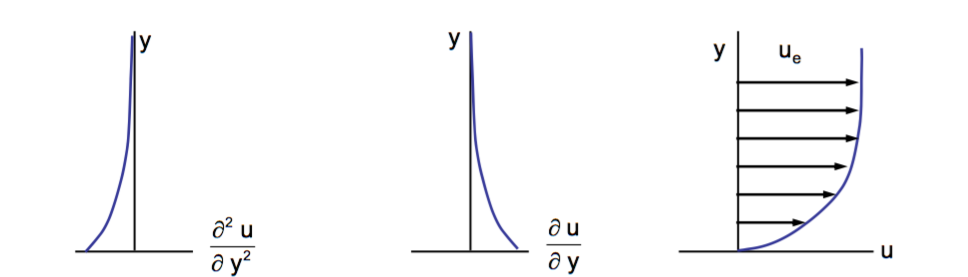
\includegraphics[width=.75\textwidth]{images/seperation_favorable_pg.png}
    \end{figure}
    \subsubsection{Zero Pressure Gradient}
    \begin{equation*}
        \frac{dp_e}{dx} = \mu \partderivtwo{u}{y} = 0
    \end{equation*}
    \begin{figure}[H]
        \centering
        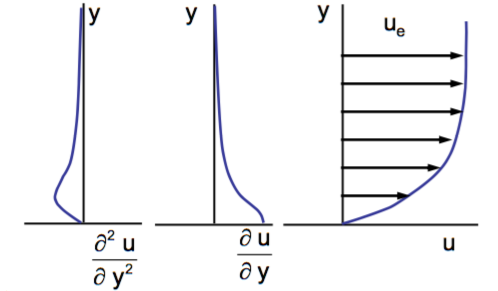
\includegraphics[width=.5\textwidth]{images/seperation_zero_pg.png}
    \end{figure}
    \subsubsection{Adverse Pressure Gradient}
    \begin{equation*}
        \frac{dp_e}{dx} = \mu \partderivtwo{u}{y} > 0
    \end{equation*}
    \begin{figure}[H]
        \centering
        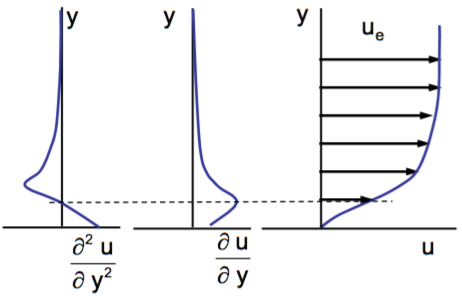
\includegraphics[width=.5\textwidth]{images/seperation_adverse1_pg.png}
    \end{figure}

    Flow separation happens when $\tau_w = \mu \partderiv{u}{y} = 0$
    \begin{figure}[H]
        \centering
        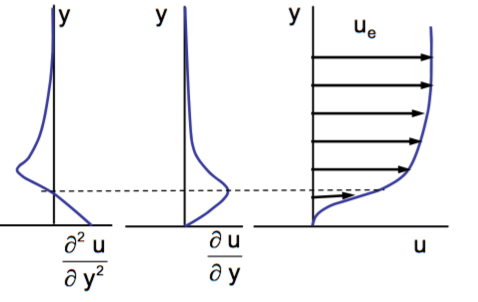
\includegraphics[width=.5\textwidth]{images/seperation_adverse2_pg.png}
    \end{figure}

    Separated flow region exists where $\tau_w = \mu \partderiv{u}{y} < 0$
    \begin{figure}[H]
        \centering
        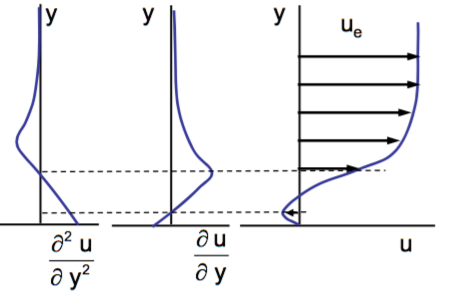
\includegraphics[width=.5\textwidth]{images/seperation_adverse3_pg.png}
    \end{figure}
    \subsection{Stagnation Flow}
    \subsubsection{Planar}
    For flow over surface of cylinder or airfoil
    \begin{itemize}
        \item Flow velocity far away approximated as $u = Bx$, $v = -By$
        \item $B$ is the strain rate at the stagnation point
        \item relevant viscous length: $\ell = \sqrt{\frac{\nu}{B}}$
        \item $x^* = x \sqrt{\frac{B}{\nu}}$, $y^* = y \sqrt{\frac{B}{\nu}}$
        \item boundary layer thickness, $\delta = 2.4 \sqrt{\frac{\nu}{B}}$, which is a constant
        \item Viscous diffusion thickens the viscous region, favorable pressure gradient (increasing speed) thins it. The two effects perfectly offset eachother
        \item $\tau_w = 1.2326 \sqrt{\rho \mu B} B x$; Grows linearly with $x$
        \item $c_f = \frac{2 \tau_w}{\rho \left( B x \right)^2}= \frac{2.465}{\sqrt{Re_x}}$; $Re_x = \frac{\rho \left(B x\right) x}{\mu} = \frac
        {U x}{\nu}$; varies with $\frac{1}{x}$
    \end{itemize}
    \subsubsection{Axisymmetric}
    This would be for when considering flow over surface of a sphere
    \begin{itemize}
        \item Flow velocity far away approximated as $u_r = Br$, $u_z = -2Br$
        \item $B$ is the strain rate at the stagnation point
        \item relevant viscous length: $\ell = \sqrt{\frac{\nu}{B}}$
        \item $z^* = z \sqrt{\frac{B}{\nu}}$
        \item boundary layer thickness, $\delta = 1.95 \sqrt{\frac{\nu}{B}}$, which is a constant
    \end{itemize}

    \subsection{Boundary Layer Transition}
    \begin{itemize}
        \item Transition Reynolds Number
        \item Critical Reynolds Number
        \item Affect of Temperature on transition
        \item Turbulent BL affect on drag
    \end{itemize}

    \subsection{Heat transfer in Boundary layers}
    \begin{itemize}
        \item Adiabatic Wall Temperature is temperature recovered through viscous heating as the flow is slowed in the boundary layer. $T_{aw} = T_{oe}$ for $Pr = 1$. This temperature rise is not gained by a stagnation type effect, but has a similar effect. 
        \item Recovery Factor related $T_{aw}$ to $T_{oe}$ as a function of $Pr$
        \item $r \simeq \sqrt{Pr} for Pr < 3.0$
        \item $r$ is not directly dependent on $Re$, but is indirectly associated with it. Increasing $Re$ implies 
        increasing $U$, all else held fixed. For a perfect gas $r \sim \frac{1}{U^2}$ and hence $r \sim \frac{1}{Re^2}$
    \end{itemize}

\section{Fundamental Equations}   
    \subsection{Continuity}
        \begin{itemize}
            \item $\partderiv{\rho}{t} + \partderiv{\rho V_i}{x_i} \\%
            \partderiv{\rho}{t} + V_i \partderiv{\rho}{x_i} + \rho \partderiv{V_i}{x_i} \\%
            \matderiv{\rho}{t} + \rho \partderiv{V_i}{x_i}$ 
            \item Incompressible, $\matderiv{\rho}{t} = 0$; $\partderiv{V_i}{x_i} = 0$
            \item $\frac{d}{dT} \iiint\limits_{\mathfrak{R}} \rho\  d\mathfrak{R} + \iint\limits_{S} \rho \vec{V} \cdot \vec{n}\  dS$
        \end{itemize}
    \subsection{Momentum} 
        \begin{itemize}
            \item $\rho \left( \partderiv{V_i}{t} + V_k \partderiv{V_i}{x_k} \right) = \rho f_i + \partderiv{\sigma_{ik}}{x_k}$
            \item $\underbrace{\rho \left( \partderiv{V_i}{t} + V_k \partderiv{V_i}{x_k} \right)}_\text{Inertia force per unit vol.} = %
            \overbrace{\rho f_i}^{\text{body force}} +%
            \underbrace{\partderiv{p}{x_i}}_\text{press. force}+%
            \overbrace{\partderiv{}{x_p}\left( \mu \left( \partderiv{V_i}{x_p} + \partderiv{V_p}{x_i} \right) + \lambda \partderiv{V_q}{x_q} \delta_{ip} \right)}^\text{viscous (friction) force per unit vol.}$ \\
            Note on Press. force per unit vol: $\partderiv{p}{x_i} = u_e \partderiv{u_e}{x_i}$
            \item $\frac{d}{dT} \iiint\limits_{\mathfrak{R}} \rho\vec{V} d\mathfrak{R} + %
            \iint\limits_{S} \left(\rho \vec{V}\right) \vec{V} \cdot \vec{n}\ dS = \iiint\limits_{\mathfrak{R}} \rho \vec{f}\ d\mathfrak{R}%
            - \iint\limits_{S} p \vec{n} dS + \iint\limits_{S} \barbelow{\tau} \cdot \vec{n}\ dS$
            \item $\sigma_{ik} = -p \delta_{ik} + \tau_{ik}$; $\tau_{ik} = 0$ for fluid at rest
        \end{itemize}
    \subsection{Energy}

\section{Nondimensionalizations}
    \subsection{High Reynolds Number Limit}
    \subsection{Low Reynolds Number Limit}

\section{Couette \& Pousille Flow} 
    \subsection{Steady}
    \subsection{Unsteady}   

\section{Creeping Flow (low Reynolds number)}

    \subsection{Flow Past Sphere}
    \begin{itemize}
        \item From potential flow: $C_p = 1 - 2.25 sin^2(\theta)$
        \item Real pressure distribution deviates because of separation
        \item subcritical flow (before turbulent transition): $Re < 2e5$, flow separated at $\theta < 90^\circ$. $Cp \simeq -.2$ in separated region
        \item supercricital flow (after turbulent transition): $Re > 2e5$, flow separated at $\theta \simeq 100^\circ$; $C_p > 0$ in separated region
    \end{itemize}
    \begin{figure}[H]
        \centering
        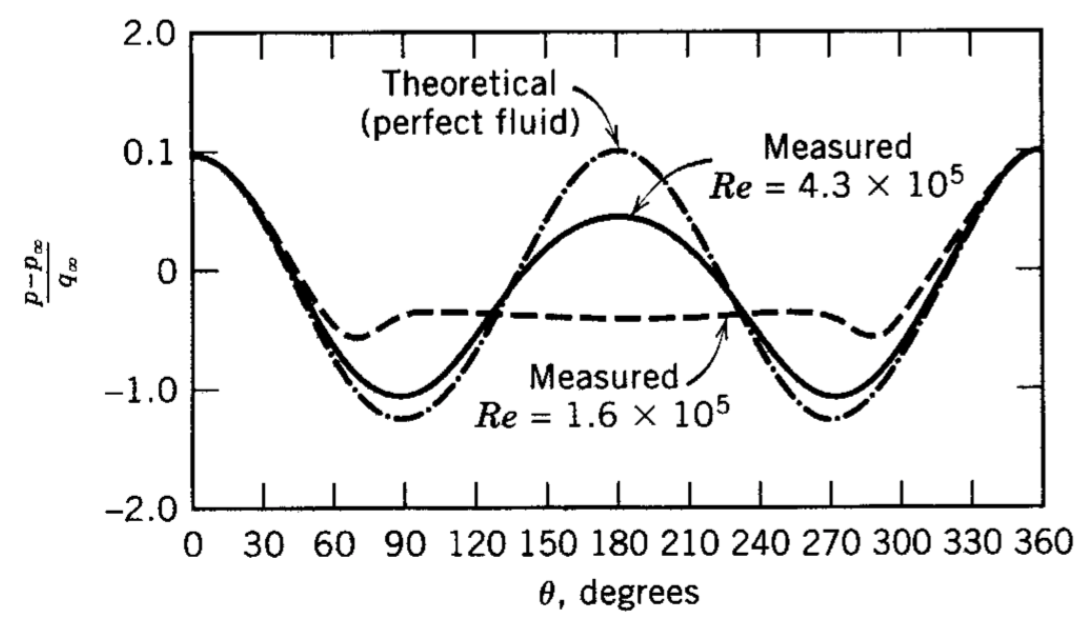
\includegraphics[width=.75\textwidth]{images/pressure_about_sphere.png}
    \end{figure}

    \subsection{Flow Past a Cylinder}
    \begin{itemize}
        \item Well defined vortex shedding region from $ \sim100 \leq Re \leq \sim4e5$
        \item coupling between vortex shedding and location of separation (not a steady separation point!)
        \item flow become turbulent when $Re > \sim 4e5$ and the wake shrinks
        \item From potential flow: $C_p = 1 - 4sin^2(\theta)$
        \item subcritical flow (before turbulent transition): $Re < 4e5$, flow separated at $\theta < 70^\circ$. $Cp \simeq -1$ in separated region
        \item supercricital flow (after turbulent transition): $Re > 4e5$, flow separated at $\theta \simeq 100^\circ$; $C_p \sim  0$ in separated region
    \end{itemize}
    \begin{figure}[H]
        \centering
        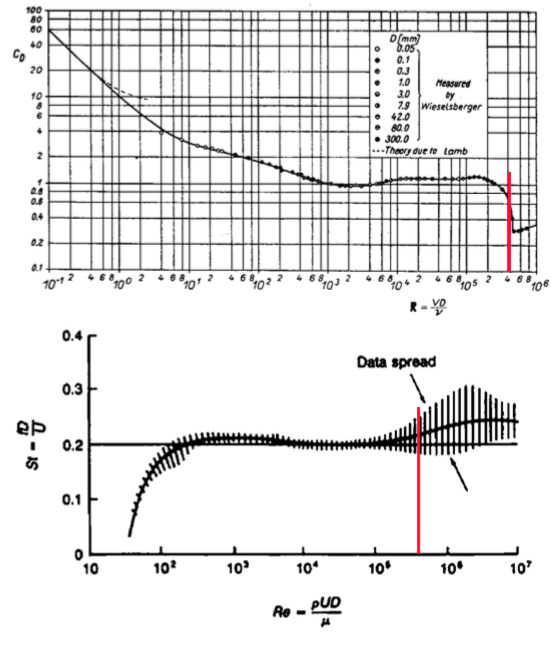
\includegraphics[width=.5\textwidth]{images/cylinder-drag-vortex-shedding.png}
    \end{figure}

\section{Laminar Boundary Layer}
    \begin{itemize}
        \item Velocity Thickness $\delta$: $u\left( y=\delta(x),x \right) = .99 u_e$
        \item Displacement Thickness: $\delta^* = \int\limits_0^\infty \left( 1 - \frac{\rho u}{\rho_e u_e} \right) dy$ \\
        (incompressible) $\delta^* = \int\limits_0^\infty \left( 1 - \frac{u}{u_e} \right) dy$
        \item Momentum Thickness: $\theta = \int\limits_0^\infty \frac{\rho u}{\rho_e u_e}\left( 1 - \frac{\rho u}{\rho_e u_e} \right) dy$
        \item Friction Coefficient: $c_f = \frac{2 \tau_w}{\rho_e u_e^2}$; $\tau_w = \mu \left.\partderiv{u}{y}\right|_{y=0}$
    \end{itemize}
    \subsection{Blassius}
        \begin{itemize}
            \item $\frac{\delta}{x} = \frac{5}{\sqrt{Re_x}}$;  $\frac{\delta^*}{x} = \frac{1.72}{\sqrt{Re_x}}$; %
            $\frac{\theta}{x} = c_f = \frac{.664}{\sqrt{Re_x}}$; 
            \item Drag per unit span for one side: $D = \frac{1.328}{\sqrt{Re_L}}$
        \end{itemize}
    \subsection{Approximate Boundary Layer Profiles}
    \subsection{Falkner Scan}
    \begin{figure}[H]
        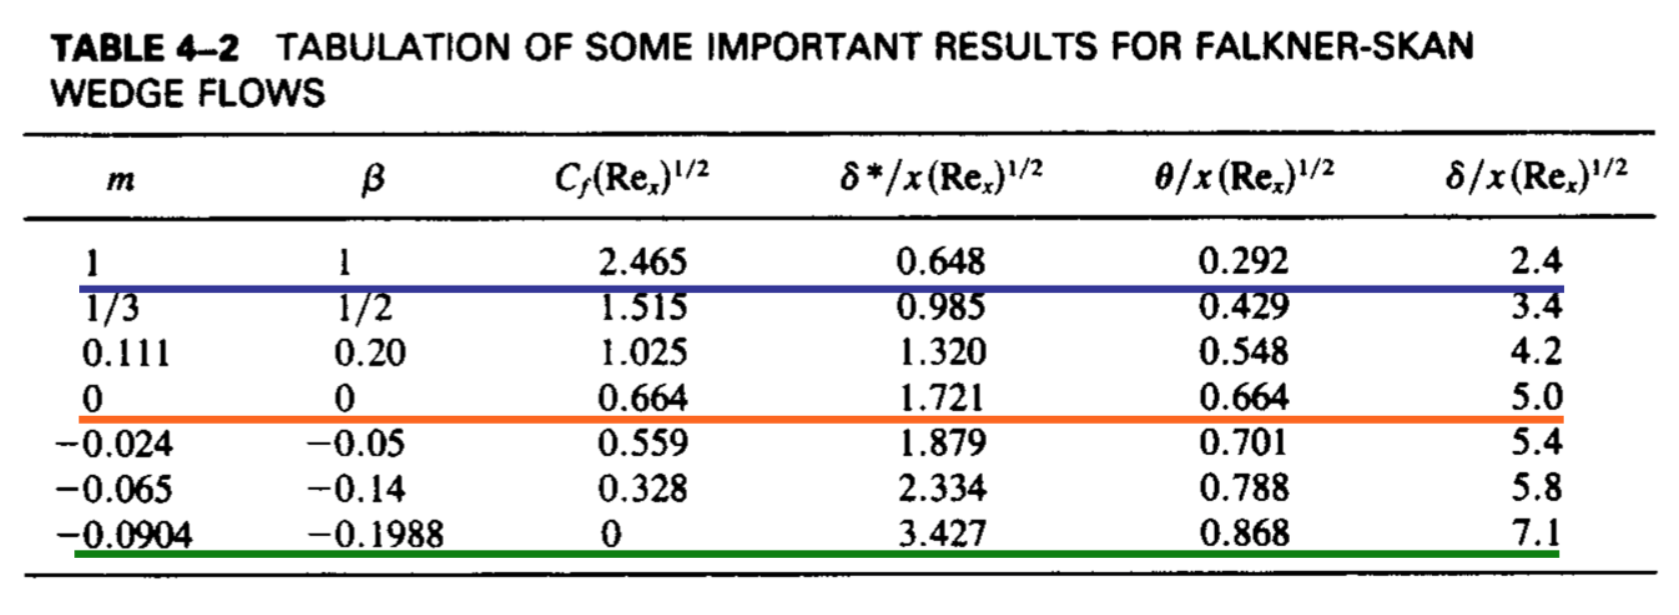
\includegraphics[width=.95\textwidth]{images/falkner_skan_table.png}
    \end{figure}
    \subsection{Thwaites Method}
    \begin{equation*}
        \frac{u_e \theta^2}{\nu} = \frac{C}{u_e^{b-1} (x)} + \frac{a}{u_e^{b-1} (x)} \int\limits_0^x u_e^{b-1}(x^\prime) dx^\prime
    \end{equation*}

    Given $F(\lambda) = a - b \lambda = .45 - 6 \lambda$; $\lambda = \frac{\theta^2}{\nu} \frac{du_e}{dx}$

    \subsubsection{Internal Flows}
        \begin{itemize}
            \item $C = \frac{u^b\theta_o^2}{\nu}$
            \item $\theta^2  = \theta_0^2 \left( \frac{u_o}{u_e(x)} \right)^6 + \frac{.45 \nu}{u_e^6(x)} \int\limits_0^x u_e^5(x^\prime) dx^\prime$
        \end{itemize}
    \subsubsection{External Flows}
        \begin{itemize}
            \item $C = 0$
            \item $\theta^2  = \frac{.45 \nu}{u_e^6(x)} \int\limits_0^x u_e^5(x^\prime) dx^\prime$
            \item at stagnation point: $\theta^2(0) = \frac{.075\nu}{\left.du_e/dx \right|_{x=0}}$
        \end{itemize}
    \subsubsection{Separation}
        \begin{itemize}
            \item $\delta^* = \theta H(\lambda)$
            \item $H(\lambda) = 2 + 4.14x - 83.5z^2 + 854z^3 - 3337z^4 + 4576z^5$ ; $z = .25 - \lambda$
            \item separation occurs when $\lambda=-.09$
        \end{itemize}

\section{Turbulent Boundary Layer}

\section{Compressible Boundary Layer}
    \subsection{Crocco-Busemann Relations}
        \begin{itemize}
            \item assumes that $Pr = 1$ (reasonable approximation for gasses with $Pr \simeq .72$)
            \item makes use of a solution $h_t = const$ throughout boundary layer. 
            \item $h_t = h + \frac{u^2}{2}$; so at wall, $u=0$, $h_t = h_w$; This means that $h_w = const$ for the solutions to hold 
        \end{itemize}

\section{Free Shear Flows}
    Laminar free shear flows are very unstable and are not commonly found in practice

    \subsection{Laminar Plane Jet}
        \begin{itemize}
            \item $J$ is jet momentum per unit width 
            \item characteristic velocity: $U_c = \sqrt{\frac{J}{\rho x}}$
            \item $Re_x \sim \frac{U_c x}{\nu} =\sqrt{\frac{J \rho x}{mu^2}}$
            \item $U_{cl} = \left(\frac{3}{32}\right)^{\frac{1}{3}} \left( \frac{J^2}{\rho \mu x} \right)^{\frac{1}{3}} %
            = .45428 \left( \frac{J^2}{\rho \mu x} \right)^{\frac{1}{3}}$
            \item 1\% velocity width: $2y \vert_{1\%} = b \simeq 21.8 \left( \frac{x^2 \mu^2}{J \rho} \right)^\frac{1}{3}$
            \item $\dot{m} = \left( 36 J \rho \mu x \right)^\frac{1}{3}$
        \end{itemize}

    \subsection{Plane Laminar Wake}
        \begin{itemize}
            \item velocity defect: $u_1$
            \item $\frac{u_1}{U_o} = C_D \left(\frac{Re_L}{16 \pi}\right)^\frac{1}{2} %
            \left( \frac{L}{x} \right)^\frac{1}{2} e^{-\frac{U_o y^2}{4x\nu}}$
            \item for a flat plate, of length $L$, wetted on both sides: $\frac{u_1}{U_o} = \frac{.664}{\sqrt{\pi}} \left( \frac{L}{x} \right)^\frac{1}{2}$
        \end{itemize}

\end{document}